% MODULO DE DISEÑO ================
    \section{Comprensión de la Situación de Comunidad Sorda en Guatemala}
    
    El análisis de mercado y el contexto guatemalteco revelaron que, aunque existen aplicaciones internacionales como Hand Talk Translator y SLAIT, ninguna se adapta a las necesidades específicas de la comunidad sorda en Guatemala, ni incluye LENSEGUA. Como resultado, se determinó la necesidad de desarrollar una solución local, específicamente diseñada para las barreras lingüísticas y culturales del país. Además, la revisión del Decreto 3-2020 confirmó la importancia de una herramienta que no solo facilite la comunicación entre sordos y oyentes, sino que también promueva el aprendizaje de LENSEGUA. Las entrevistas realizadas a personas sordas y a individuos en constante contacto con la comunidad sorda, junto con encuestas dirigidas a personas oyentes, subrayaron de manera contundente la necesidad de esta aplicación. Se evidenció que las barreras para las personas sordas en Guatemala son significativas y que existe un considerable desconocimiento sobre LENSEGUA, dado que el 70\% de los encuestados reconoció no estar familiarizado con esta lengua. Esta información recalca la urgencia de desarrollar una herramienta diseñada específicamente para atender estas deficiencias.
    
    \section{Diseño Centrado en el Usuario}
    
    El diseño de la aplicación fue un proceso iterativo basado en varias herramientas de diseño, como mapas de empatía, personas, diagramas de afinidad y flujos de usuario. Este proceso dio como resultado un prototipo interactivo de alto nivel desarrollado en Figma. Dicho prototipo permitió definir de manera clara la navegación y la experiencia del usuario. El prototipo integró las recomendaciones de asociaciones como En-Señas y expertos en diseño, lo que aseguró que la aplicación no solo fuera funcional, sino también accesible y fácil de usar para la comunidad sorda. 

    
    \section{Desarrollo de Aplicación Móvil para Android}
    
    El desarrollo de la aplicación fue llevado a cabo utilizando una arquitectura modular basada en el patrón MVVM, lo que permitió que la aplicación fuera fácilmente escalable y mantenible. Se implementaron componentes reutilizables, lo que aumentó la eficiencia en el desarrollo, reduciendo la redundancia en el código. Además, se integraron diversas librerías que optimizaron el rendimiento general de la aplicación. El uso de Kanban durante el desarrollo facilitó una gestión eficaz de las tareas, asegurando que se cumplieran los plazos y que las funcionalidades clave se implementaran correctamente. El desarrollo resultó en una versión funcional de la aplicación lanzada en fase de prueba cerrada en \textit{Play Store}, lo que permitió a un grupo selecto de usuarios interactuar con ella antes de su lanzamiento oficial. 


    \section{Pruebas con Usuarios Exitosas}
    
    Durante las pruebas, se presentaron los flujos críticos de la aplicación en eventos clave como la Expo UVG y una presentación especial con la asociación En-Señas. El resultado de estas pruebas fue altamente positivo, ya que los usuarios destacaron la intuitividad y facilidad de uso de la aplicación. Se registró un 90\% de éxito en las pruebas de usabilidad con En-Señas, en las cuales los usuarios pudieron completar tareas clave como la creación de cuentas, grabación de videos y traducción de señas sin dificultades importantes. Estas pruebas confirmaron que la aplicación era funcional, accesible y cumplía con las expectativas de los usuarios, demostrando cómo la investigación, el diseño y el desarrollo se integraron armoniosamente para formar un producto final exitoso. Esto reafirma que cada fase fue ejecutada correctamente, contribuyendo al logro de un resultado sólido y coherente.
    
% MODULO DE ARQUITECTURA DE RED ==========

\section{Redireccionamiento de puertos para acceso SSH Externo}

Una vez asignados los recursos, se procede a la configuración de la red y acceso remoto para cada máquina virtual. Mediante la implementación de reglas de redireccionamiento de puertos \textbf{con iptables}, se permite el acceso a las VMs desde el exterior a través de SSH. Cada máquina virtual se ha configurado para ser accesible mediante un puerto específico: \textbf{2222 para VM1}, \textbf{2223 para VM2} y \textbf{2224 para VM3}. Este esquema de puertos permite una administración centralizada y segura desde cualquier ubicación externa, sin necesidad de modificar la configuración interna de las VMs.

\begin{itemize}
    \item \textbf{Para VM1 (puerto 2222)}
    \begin{itemize}
        \item \texttt{sudo iptables -t nat -A PREROUTING -p tcp --dport 2222 -j \newline
        DNAT --to-destination 10.47.92.160:22}
        
        \item \texttt{sudo iptables -t nat -A POSTROUTING -p tcp -d 10.47.92.160 \newline
        --dport 22 -j MASQUERADE}
    \end{itemize}
    
    \item \textbf{Para VM2 (puerto 2223)}
    \begin{itemize}
        \item \texttt{sudo iptables -t nat -A PREROUTING -p tcp --dport 2223 -j \newline
        DNAT --to-destination 10.47.92.70:22}
        
        \item \texttt{sudo iptables -t nat -A POSTROUTING -p tcp -d 10.47.92.70 \newline
        --dport 22 -j MASQUERADE}
    \end{itemize}
    
    \item \textbf{Para VM3 (puerto 2224)}
    \begin{itemize}
        \item \texttt{sudo iptables -t nat -A PREROUTING -p tcp --dport 2224 -j \newline
        DNAT --to-destination 10.47.92.195:22}
        
        \item \texttt{sudo iptables -t nat -A POSTROUTING -p tcp -d 10.47.92.195 \newline
        --dport 22 -j MASQUERADE}
    \end{itemize}
\end{itemize}


Estas reglas fueron guardadas y aplicadas de manera persistente para asegurar su disponibilidad tras cualquier reinicio. El acceso SSH se configuró adicionalmente para utilizar claves públicas generadas desde sistemas Windows, facilitando una autenticación segura y sin contraseña.

En cuanto a la seguridad de las bases de datos, se decidió utilizar MySQL Server, gestionando la contraseña del usuario root para fortalecer la protección. El comando \texttt{ALTER USER} fue utilizado para actualizar la contraseña y asegurar que el acceso sea exclusivo desde el host local, minimizando riesgos.

Esta metodología garantiza una infraestructura virtualizada sólida, segura y eficiente, diseñada para soportar altas demandas y mantener la estabilidad bajo cargas intensivas.

\section{Resultados de la Prueba de Carga}

Para evaluar el rendimiento del servidor, se realizaron pruebas de carga con un número creciente de usuarios concurrentes. A continuación, se presentan los resultados obtenidos y las métricas de rendimiento observadas.

\begin{figure}[H]
    \centering
    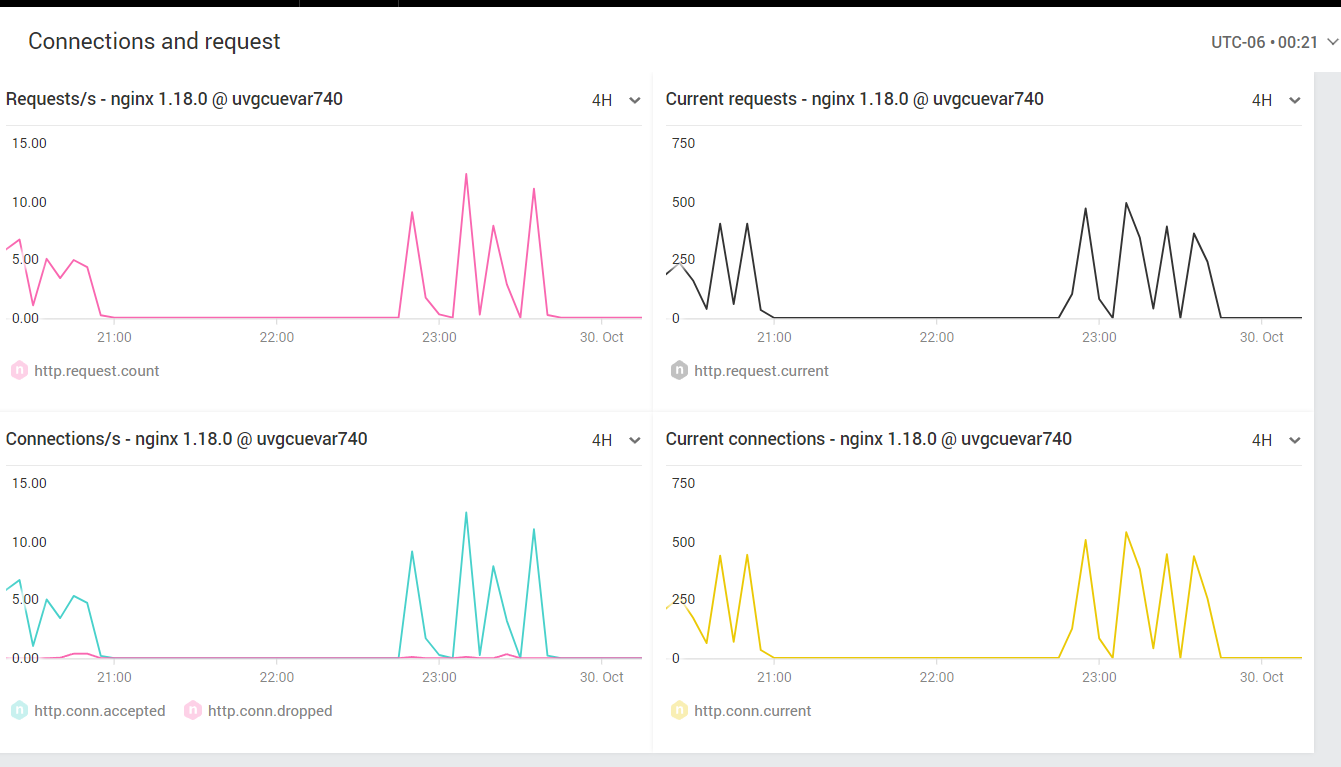
\includegraphics[width=0.8\textwidth]{figuras/ConnectionsAndRequest.png}
    \caption{Métricas de Conexiones y Solicitudes: Requests/s y Conexiones Actuales}
    \label{fig:connectionsAndRequest}
\end{figure}

\paragraph{Requests/s y Conexiones Actuales}
El servidor mostró un buen manejo de solicitudes por segundo (requests/s), manteniendo una cantidad de peticiones estable hasta las pruebas con una carga elevada. Esto demuestra que la configuración de NGINX y Gunicorn está bien ajustada para recibir y gestionar una alta cantidad de solicitudes concurrentes. Los picos de conexiones actuales también son gestionados adecuadamente, lo que indica que NGINX puede aceptar múltiples conexiones sin saturarse. La configuración con Gunicorn, que permite manejar conexiones asincrónicas y de múltiples hilos, ayuda a procesar solicitudes de manera eficiente y a mantener baja la latencia.

\begin{figure}[H]
    \centering
    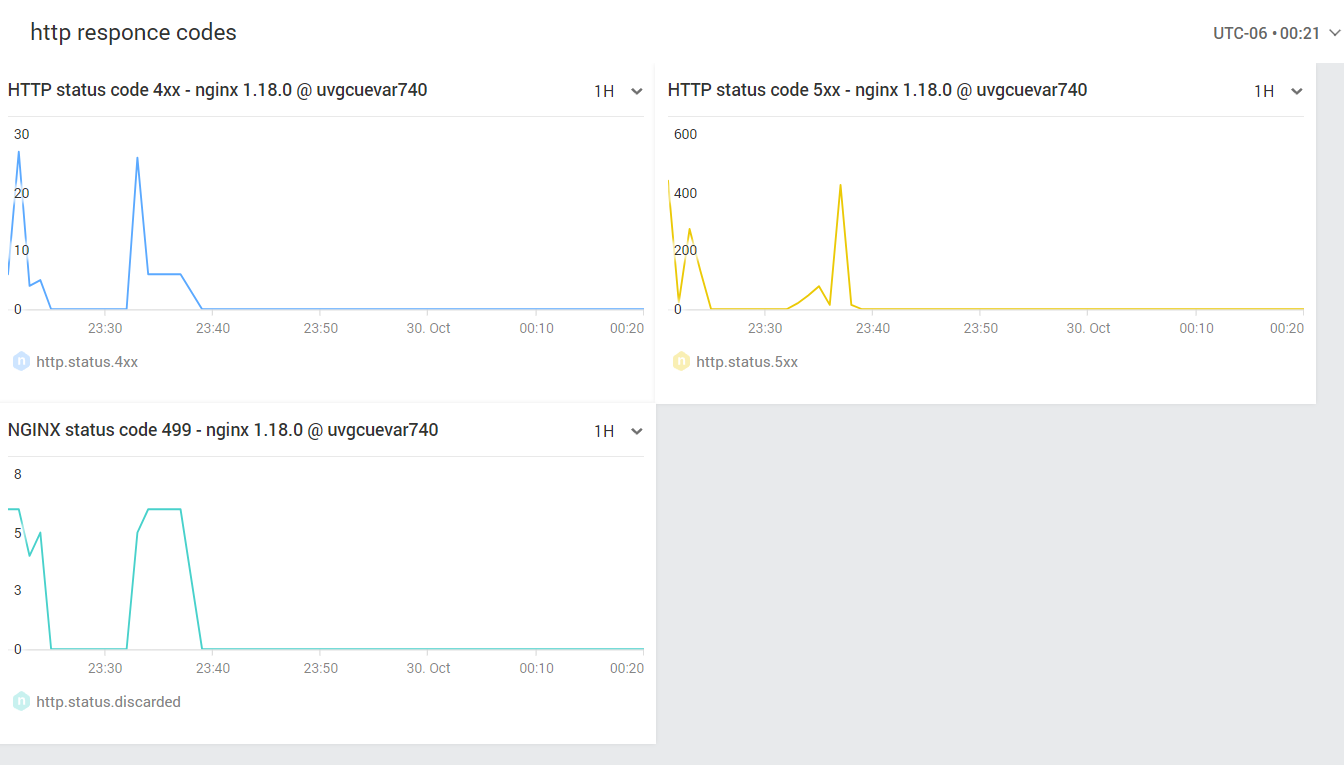
\includegraphics[width=0.8\textwidth]{figuras/HttpResponceCodes.png}
    \caption{Códigos de Respuesta HTTP}
    \label{fig:httpResponceCodes}
\end{figure}

\paragraph{Códigos de Respuesta HTTP}
A medida que la carga se incrementó, comenzaron a aparecer errores 4xx y 5xx, particularmente en las pruebas de 500 usuarios en adelante. Sin embargo, los errores no fueron críticos y no afectaron significativamente el desempeño general del sistema. Esto sugiere que el sistema maneja bien la mayoría de las solicitudes válidas, y los errores observados son principalmente resultado de una sobrecarga extrema y no de una falla en la configuración de NGINX o Gunicorn. Los errores 499 indican que algunos clientes abandonaron la conexión antes de recibir respuesta, lo cual puede deberse a tiempos de respuesta más largos bajo carga alta.

\begin{figure}[H]
    \centering
    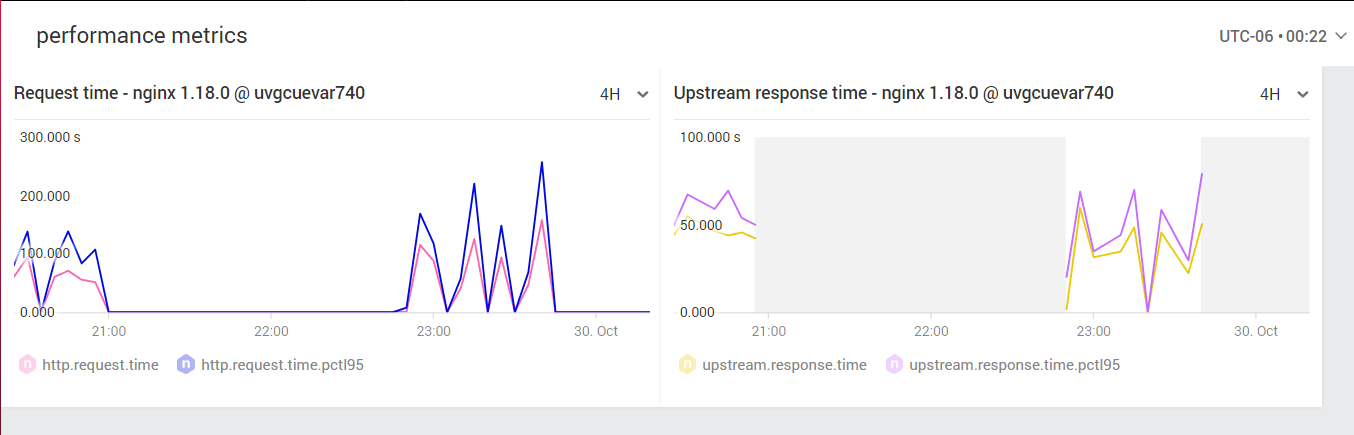
\includegraphics[width=0.8\textwidth]{figuras/PerformanceMetrics.png}
    \caption{Tiempo de Respuesta y Tiempo de Respuesta Upstream}
    \label{fig:performanceMetrics}
\end{figure}

\newpage

\paragraph{Tiempo de Respuesta y Tiempo de Respuesta Upstream}
Los tiempos de respuesta aumentaron bajo cargas intensas, pero se mantuvieron razonablemente estables hasta los niveles de carga de 400-500 usuarios. Esto demuestra que la arquitectura NGINX-Gunicorn-Flask es capaz de manejar eficientemente el procesamiento de las solicitudes hasta un nivel considerable de concurrencia. A pesar de algunos picos, los tiempos de respuesta hacia los servicios backend (upstream) fueron manejados adecuadamente, lo que muestra que la configuración de Gunicorn en conjunto con Flask está optimizada para responder rápidamente.

\begin{figure}[H]
    \centering
    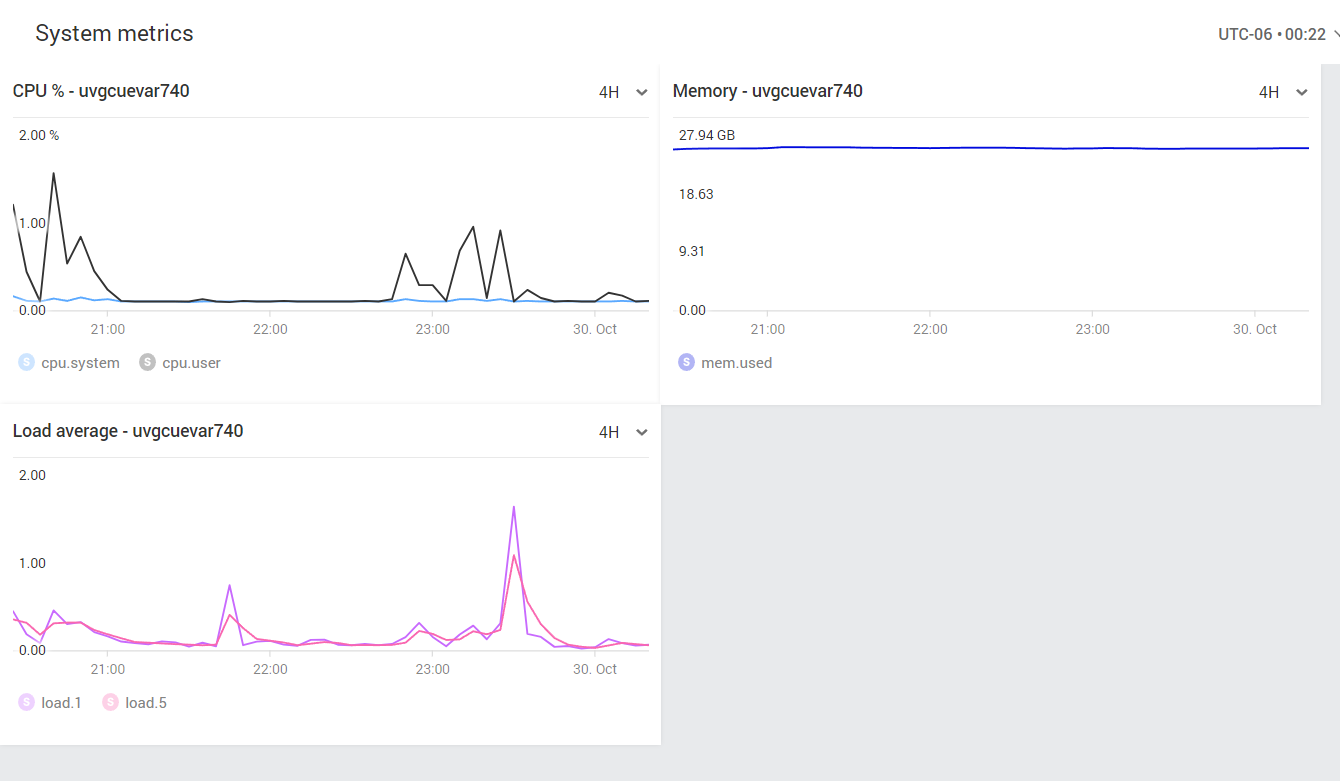
\includegraphics[width=0.8\textwidth]{figuras/SystemMetrics.png}
    \caption{Métricas de CPU, Memoria y Carga del Sistema}
    \label{fig:systemMetrics}
\end{figure}

\paragraph{CPU, Memoria y Carga del Sistema}
Aunque se observan picos en el uso de CPU bajo carga intensa, el sistema utilizó eficientemente los recursos de CPU proporcionados (32 CPUs en total), manteniendo un uso moderado incluso en las pruebas con cargas más altas. Esto muestra que el sistema distribuye eficientemente las solicitudes entre los hilos de Gunicorn, sin sobrecargar los recursos de CPU. El uso de memoria se mantuvo bajo, lo cual es un indicativo de una configuración optimizada para el consumo de memoria. El load average del sistema permaneció dentro de límites aceptables, indicando capacidad para gestionar volúmenes de carga sin requerir ajustes adicionales.

\begin{figure}[H]
    \centering
    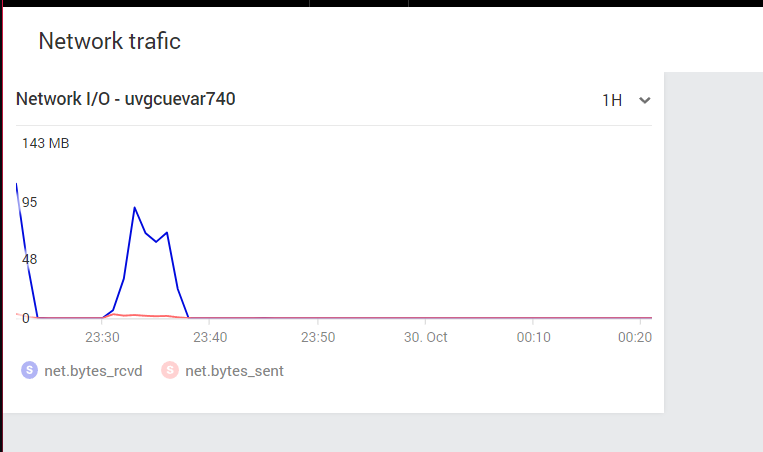
\includegraphics[width=0.8\textwidth]{figuras/NetworkTraffic.png}
    \caption{Tráfico de Red (Network I/O)}
    \label{fig:networkTraffic}
\end{figure}

\paragraph{Tráfico de Red}
El tráfico de red aumentó durante las pruebas de carga, particularmente en el tráfico recibido (\texttt{net.bytes\_rcvd}), lo cual es esperado debido al incremento de solicitudes. NGINX manejó eficientemente el enrutamiento de solicitudes y respuestas a través de la red, incluso a través de la VPN de la universidad, lo cual muestra que la configuración es robusta en entornos con restricciones de red.

\paragraph{Resumen de Desempeño y Justificación}
En general, el sistema basado en NGINX, Gunicorn y Flask ha demostrado ser eficiente y efectivo para manejar solicitudes concurrentes bajo una variedad de cargas. Las métricas muestran que el sistema puede manejar hasta aproximadamente 400-500 usuarios concurrentes sin problemas mayores, mientras que las pruebas de carga más altas empiezan a mostrar signos de saturación. La configuración actual es adecuada para el entorno de red restringido de la universidad y demuestra estabilidad en condiciones de carga media-alta.

\section{Resultados de la Prueba E2E}
Los resultados de esta prueba demostraron un éxito del 100\%, ya que cada API involucrada respondió adecuadamente en el flujo esperado. La prueba incluyó las siguientes operaciones:
\begin{itemize}
    \item Registro de usuario.
    \item Inicio de sesión.
    \item Consulta de información de perfil.
    \item Envío de video.
    \item Marcado y desmarcado del video como favorito.
    \item Envío de una traducción.
    \item Marcado y desmarcado de la traducción como favorita.
    \item Incremento de la racha de actividad (streak).
\end{itemize}

Cada una de estas operaciones se ejecutó sin errores, y los tiempos de respuesta se mantuvieron dentro de los niveles aceptables, garantizando la correcta integración de los diferentes módulos del sistema.

\begin{figure}[H]
    \centering
    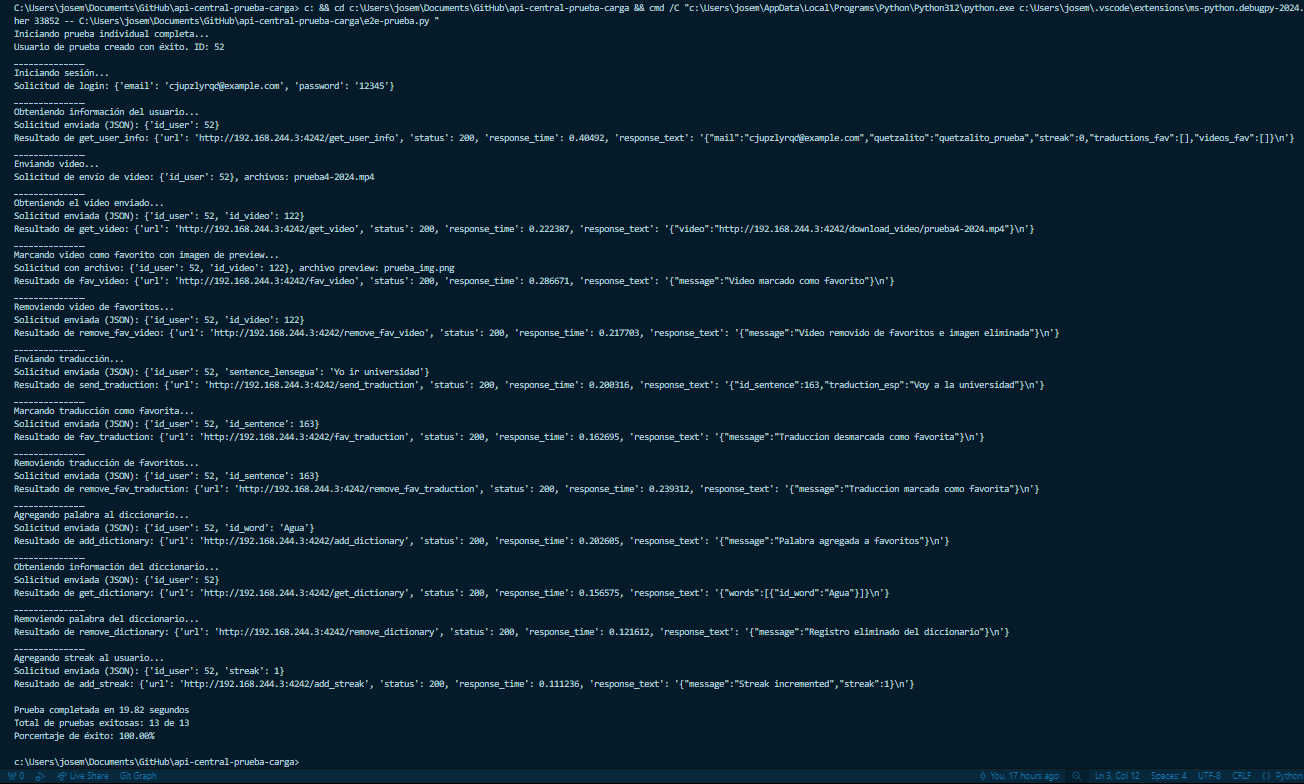
\includegraphics[width=0.5\textwidth]{figuras/e2etest.png}
    \caption{Resultados de la prueba E2E, mostrando un 100\% de éxito en todas las operaciones realizadas.}
    \label{fig:e2etest}
\end{figure}

\section{Resultados de la Prueba de Seguridad con Lynis}

Para evaluar la seguridad de nuestro sistema, utilizamos Lynis, una herramienta de auditoría que examina la configuración del sistema, busca vulnerabilidades y proporciona un índice de robustez conocido como el "Hardening Index". Lynis es ampliamente utilizado en sistemas UNIX y Linux para evaluar y mejorar la seguridad del sistema. Los resultados de la prueba realizada en nuestro servidor se muestran en la Figura~\ref{fig:primeraPruebaLynis}.

\begin{figure}[H]
    \centering
    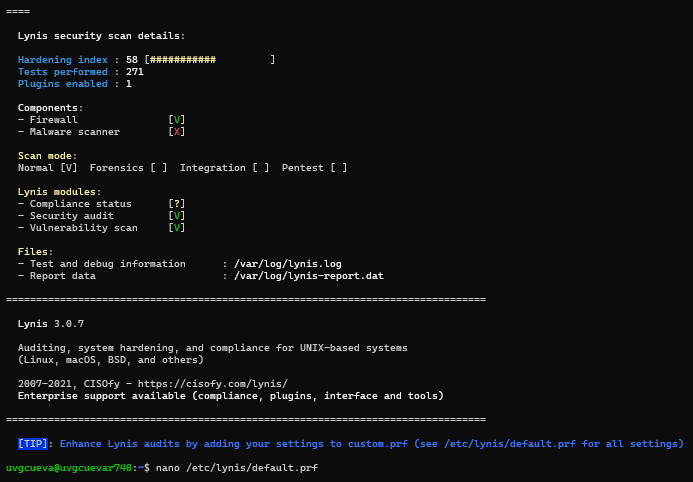
\includegraphics[width=0.7\textwidth]{figuras/primeraPruebaLynis.png}
    \caption{Resultado de la primera prueba de seguridad con Lynis mostrando un índice de robustez de 58.}
    \label{fig:primeraPruebaLynis}
\end{figure}

Durante esta primera ejecución, obtuvimos un "Hardening Index" de 58. Según la documentación de Lynis y opiniones de expertos en foros de seguridad, un índice de robustez de 50 o superior indica que el sistema es seguro, aunque siempre hay áreas que podrían beneficiarse de mejoras adicionales. Este resultado nos da confianza en la configuración actual del sistema, aunque decidimos realizar ajustes adicionales para elevar este puntaje en pruebas posteriores.

\begin{figure}[H]
    \centering
    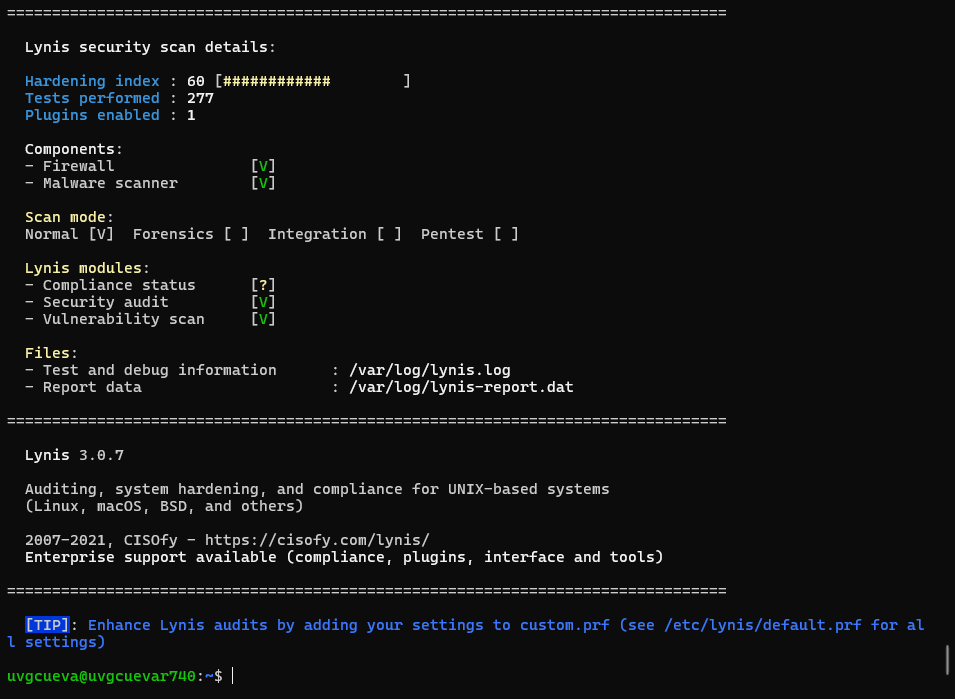
\includegraphics[width=0.7\textwidth]{figuras/segundaPruebaLynis.png}
    \caption{Resultado de la segunda prueba de seguridad con Lynis mostrando un índice de robustez de 60.}
    \label{fig:segundaPruebaLynis}
\end{figure}

La Figura~\ref{fig:segundaPruebaLynis} muestra el resultado de nuestra segunda ejecución de Lynis después de aplicar mejoras recomendadas en la configuración del sistema. En esta segunda prueba, el índice de robustez aumentó a 60, lo que demuestra que las optimizaciones realizadas han mejorado la seguridad del servidor. En general, se considera que Lynis ofrece mejores resultados en sistemas basados en Fedora, donde las configuraciones de seguridad predeterminadas están más alineadas con las recomendaciones de la herramienta.

\begin{figure}[H]
    \centering
    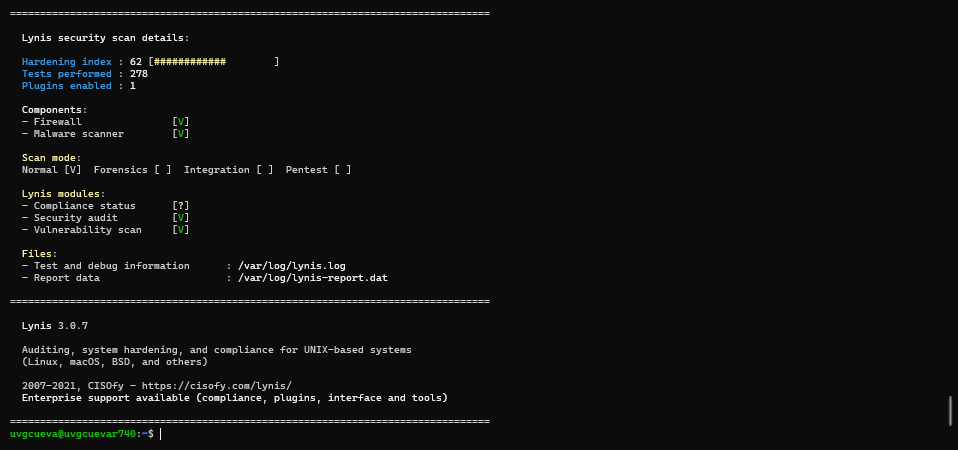
\includegraphics[width=0.7\textwidth]{figuras/terceraPruebaLynis.png}
    \caption{Resultado de la tercera prueba de seguridad con Lynis mostrando un índice de robustez de 62.}
    \label{fig:terceraPruebaLynis}
\end{figure}

En la Figura~\ref{fig:terceraPruebaLynis}, se observa el resultado de la tercera y última prueba, donde auditoría realizada con Lynis arrojó un puntaje de 62, superando significativamente la meta establecida de 40. Este resultado demostró que el sistema implementó medidas de seguridad suficientes para su propósito. Lynis, en su configuración básica y sin personalización, evaluó rigurosamente las configuraciones del sistema y detectó áreas críticas que necesitaron atención. Es importante destacar que este puntaje reflejó un sistema seguro que no había sido ajustado para ignorar reglas no aplicables a nuestro entorno, lo cual reforzó la validez del resultado obtenido. Según el artículo Lynis hardening index \cite{LynisHardeningIndex} publicado en Linux Audit, un puntaje entre 50 y 70 indica un sistema razonablemente fortalecido, ideal para aplicaciones. Este puntaje, sin configuraciones personalizadas, representó un sistema confiable y demostró que las medidas implementadas fueron más que adecuadas para el contexto en el que se desarrolló el proyecto.

\begin{figure}[H]
    \centering
    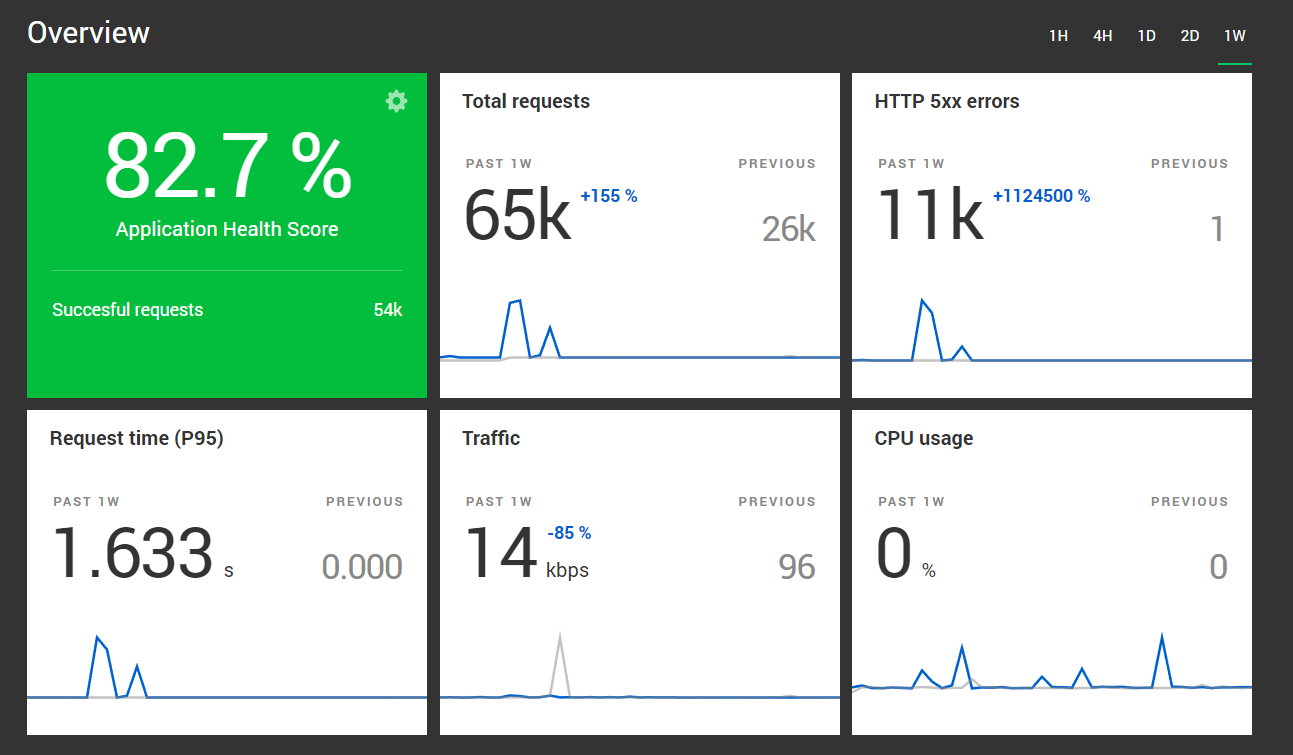
\includegraphics[width=0.8\textwidth]{figuras/OverviewServerStatus.png}
    \caption{Resumen del estado del servidor.}
    \label{fig:overview}
\end{figure}

En base a las evaluaciones de seguridad, carga y pruebas de extremo a extremo (E2E), el sistema muestra un buen estado general (Figura~\ref{fig:overview}). El \textit{Application Health Score} es de 82.7\%, con un tiempo de respuesta promedio de 1.633 segundos, indicando una respuesta rápida y estable en la mayoría de las solicitudes. Aunque se registraron algunos errores HTTP 5xx, el uso de CPU se mantuvo bajo, reflejando una buena eficiencia en el manejo de recursos.




% MODULO DE VISION POR COMPUTADORA ====





% MODULO DE CHATPGPT ====





% MODULO DE LAMDA ====